\subsubsection{K-Means}
\label{subsubsection:kmeans}
K-Means is simple and reasonably fast clustering algorithm where K represents the number of cluster the algorithm should create and means refers to the average value of each cluster. Given a set of data samples their similarity is measured as the value of the Euclidean distance between them. The general form of the Euclidean distance formula is described in equation \ref{eq:euclid}, where $p$ and $q$ represent n-dimensional feature vectors. As the K-means algorithm executes, data samples are assigned to the cluster whose average value, also as a cluster centroid, is closest to the sample's own. Centroids are updated after each round of assignments until their values converge. Initially the each cluster centroid is randomly selected. The algorithm to implement the K-means method is outlined in algorithm \ref{algorithm:kmeans}.

\begin{equation}
    EuclideanDistance(p,q) = \sqrt{(p_1 - q_1)^2 + (p_2 - q_2)^2 +\hdots + (p_n - q_n)^2}
    \label{eq:euclid}
\end{equation} 

\begin{algorithm}
    \SetAlgoLined
    \KwInput{Set of data vectors X of size M} 
    \KwOutput{K sets of clustered data vectors}
    Initialize the desired number of clusters $K$\;
    Initialize a list of $K$ random cluster centroids $\mu$\;
    \While{$\mu$ elements have not converged}{
        \For{i = 0 to M}
        {
            distOld = $\inf$
            \For{j = 0 to K}{
                distnew = EuclideanDistance(X[i], $\mu[j]$)\;
                \If{distNew $<$ distOld}{
                    distOld = distNew\;
                    $\mu_j$.append(X[i])\;
                }
            }
        }
        \For{p = 0 to K}{
            centroidList.append(average($\mu[p]$))\;
        }
    }
    \caption{K Means Clustering \cite{oreilly_python}}
    \label{algorithm:kmeans}
\end{algorithm}

The best result for this method is defined as having the smallest intra-cluster variance. K-Means is disadvantaged by the implicit trait that it formulates clusters of similar sizes. This happens because the algorithm seeks to minimize variance (spread) in each cluster hence the \q{ideal} centroid placement will form distributions spherically about centroids. Figure \ref{fig:clusters} visualizes an example of clustering data where it can be observed that the cluster sizes are similar and spherical in shape. This method of clustering does not consider any probabilistic model in classifying data, this type of classification is called a \emph{hard assignment} because a data sample can belong only to one cluster. The dual of this is a \emph{soft assignment}, considers the \emph{probability} of a sample of belonging each cluster. 

\begin{figure}[H]
    \centering
    \centering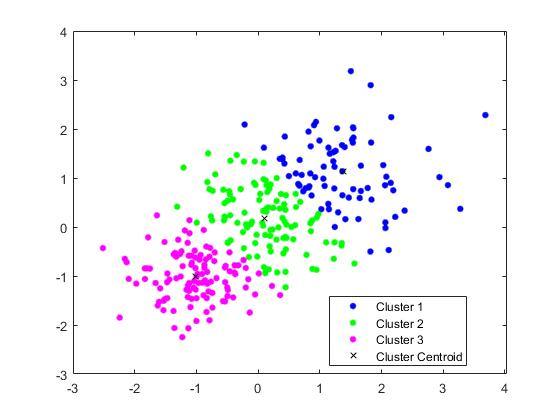
\includegraphics[width=0.9\textwidth]{kmeans_clusters}
    \caption{K-Means clustering performed on random data. \cite{matlab_clustering}}
    \label{fig:clusters}
\end{figure} 